\section{Murmuration of Modular Forms}
\label{sec:modform}

The first murmuration density that is computed ever is for modular forms by Zubrilina \cite{zubrilina2025murmurations}.
For each fixed weight $k$, she computed the murmuration density of weight $k$ cusp newforms of level $\Gamma_0(N)$, as $N \to \infty$.
In this section, we briefly sketch the main ideas and results of her work.

\subsection{Statement}

Before we state the result, we define some notations first.
For each $k$ and $N \ge 1$, let $H^{\mathrm{new}}(N, k)$ be the set of normalized Hecke cuspforms of weight $k$ and level $\Gamma_0(N)$.
For each $f \in H^{\mathrm{new}}(N, k)$, let $\epsilon(f) \in \{\pm 1\}$ be the root number of $f$, and $a_f(p)$ be the $p$-th Fourier coefficient of $f$ and $\lambda_f(p) := a_f(p) / p^{\frac{k-1}{2}}$ be its analytic normalization.
For $n \in \bZ_{\ge 0}$, \emph{$n$-th Chebyshev polynomial of the second kind} is defined as
\[
    U_n(\cos \theta) = \frac{\sin((n+1) \theta)}{\sin\theta}. 
\]
For each $r \in \bZ_{\ge 1}$, define
\[
    \nu(r) := \prod_{p | r} \left(1 + \frac{p^2}{p^4 - 2p^2 - p + 1}\right)
\]
Lastly, we define the constants $\alpha, \beta, \gamma$ as
\begin{align*}
    \alpha := 2\pi \prod_{p} \frac{p^4 - 2p^2 - p + 1}{p^4 - 2p^2 + p}, \quad
    \beta := 2\pi \prod_{p} \frac{p^3 + p^2 - 1}{p(p^2 + p - 1)}, \quad
    \gamma := 12 \prod_{p} \frac{p(p + 1)}{p^2 + p - 1}.
\end{align*}
\begin{theorem}[Zubrilina {\cite[Theorem 1]{zubrilina2025murmurations}}]
    \label{thm:zubrilina_modform}
    Let $X, Y, P$ be parameters going infinite with $X, Y > 0$ and $P$ prime; assume further that $Y = (1 + o(1))X^{1 - \delta_2}$ and $P \ll X^{1 + \delta_1}$ for some $\delta_1, \delta_2$ with $0 < \delta_1 < \frac{1}{11}, 2\delta_1 < \delta_2 < \frac{1}{13}(4 - 18 \delta_1)$.
    Let $y = P/X$. Then
    \begin{equation}
        \label{eqn:zubrilina_modform}
        \bE_{\substack{N \in [X, X + Y] \\ f\in H^{\new}(N, k)}} [\sqrt{P} \lambda_f(P) \epsilon(f)] = \frac{\sum_{N \in [X, X + Y]}^\square \sum_{f \in H^{\new}(N, k)} \sqrt{P} \lambda_f(P) \varepsilon(f)}{\sum_{N \in  [X, X + Y]}^\square \sum_{f \in H^{\new}(N, k)} 1} = \cM_k(y) + O_\varepsilon \left(X^{-\delta' + \varepsilon} + \frac{1}{P}\right)
    \end{equation}
    where
    \begin{equation}
        \cM_k(y) = \frac{\alpha(-1)^{k/2 - 1}}{k - 1} \sum_{1 \le r \le 2\sqrt{y}} \nu(r) \sqrt{4y - r^2} U_{k - 2} \left(\frac{r}{2\sqrt{y}}\right) + \frac{\beta}{k-1} \sqrt{y} - \gamma \delta_{k=2} y.
    \end{equation}
    Here $\delta' > 0$ is a constant explicitly expressible through $\delta_1, \delta_2$.
    The notation $\sum^\square$ means the sum is over square-free integers.
\end{theorem}

Figure \ref{fig:zub_Mk} shows the graphs of $\cM_k(y)$ for $k = 2, 8, 24$ (note that $U_0(x) = 1$ and $\cM_2(y)$ is a linear combination of the functions of the form $\sqrt{4y - r^2}$).
They are continuous but not differentiable at $y = \frac{r^2}{4}$ for $r \in \bZ_{>0}$, which are the points where the summation index $r$ changes.

\begin{figure}[htp] 
\centering
    \begin{subfigure}{1.0\textwidth}
        \centering
        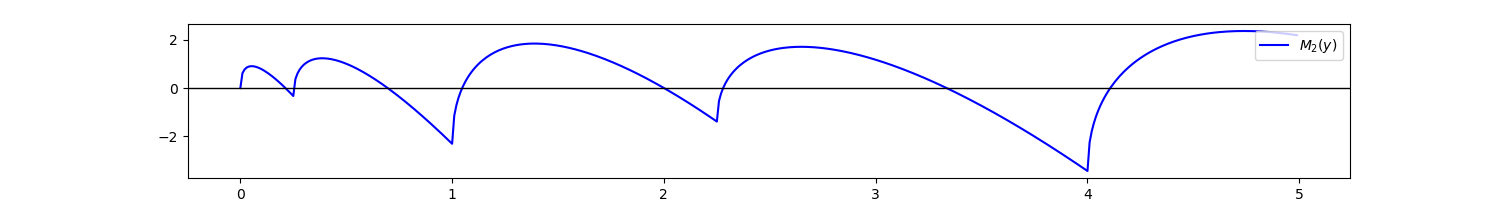
\includegraphics[width=\textwidth]{src/zub_k=2.png}%
        \label{fig:M2}
    \end{subfigure}
    
    \begin{subfigure}{1.0\textwidth}
        \centering
        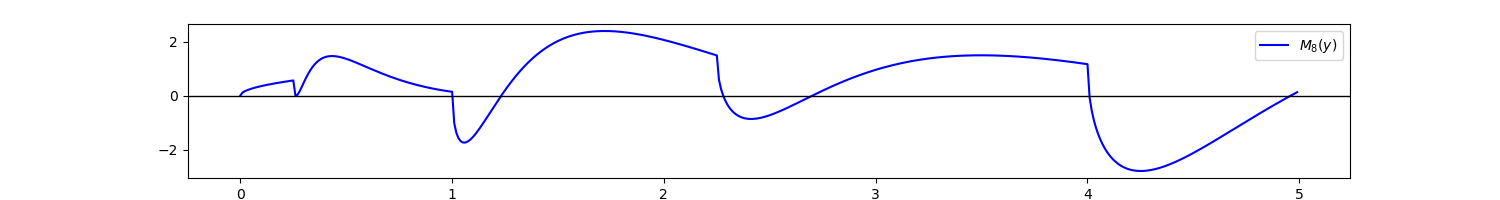
\includegraphics[width=\textwidth]{src/zub_k=8.png}%
        \label{fig:M8}
    \end{subfigure}

    \begin{subfigure}{1.0\textwidth}
        \centering
        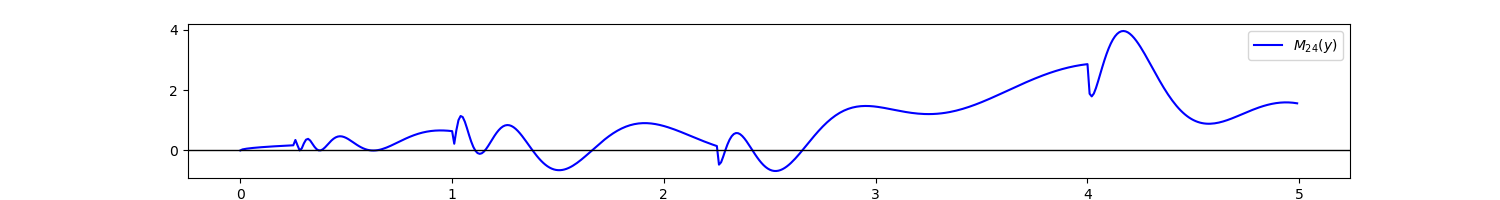
\includegraphics[width=\textwidth]{src/zub_k=24.png}%
        \label{fig:M24}
    \end{subfigure}
    
    \caption{Murmuration density $\cM_k(y)$ of modular forms for $k = 2, 8, 24$.}
\label{fig:zub_Mk}
\end{figure}


\subsection{Eichler--Selberg trace formula}

To prove Theorem \ref{thm:zubrilina_modform}, one need to understand how to estimate the numerator on the LHS.
Recall that $a_f(P)$ is the $P$-th Fourier coefficient of $f$, which is also the eigenvalue of the Hecke operator $T_P$ acting on $f$.
Also, $(-1)^{k/2}\varepsilon(f)$ is equal to the eigenvalue of the Atkin--Lehner involution $W_N = T_N$ acting on $f$.
Thus the sum appears in the numerator of LHS of \eqref{eqn:zubrilina_modform} can be interpreted as the trace of the operator $(-1)^{k/2} T_P \circ W_N$ acting on the space of cusp forms of weight $k$ and level $N$ (multiplied by $P^{1 - k/2}$).
Eichler \cite{eichler1955class} studied such a sum of traces and proved that it can be expressed in terms of (Hurwitz) class numbers, which is generalized by Selberg \cite{selberg1956harmonic}.
To account the root number $\varepsilon(f)$, i.e. eigenvalue of $W_N$, we used the following version of Eichler--Selberg trace formula by Skoruppa and Zagier \cite{skoruppa1987jacobi}.

\begin{theorem}[Skoruppa--Zagier \cite{skoruppa1987jacobi}]
    \label{thm:sz_tf}
    For square-free $N$ and prime $P \nmid N$,
    \begin{align*}
        &\sum_{f \in H^\new(N, k)} \sqrt{P} \lambda_f(P) \varepsilon(f)\nonumber \\
        &= \frac{H_1(-4PN)}{2} + (-1)^{k/2 - 1} U_{k - 2} \left(\frac{r\sqrt{N}}{2\sqrt{P}}\right) \sum_{0 < r \le 2\sqrt{P/N}} H_1(r^2 N^2 - 4PN) - \delta_{k=2}(P+1)
    \end{align*}
    Here $H_1(-d)$ ($d > 0$) is the Hurwitz class number, the number of equivalence classes of positive definite binary quadratic forms of discriminant $-d$ weighted by the number of automorphisms, i.e. with forms correspond to $x^2 + y^2$ or $x^2 + xy + y^2$ counted with multiplicity $1/2$ and $1/3$ respectively.
\end{theorem}

Hurwitz class number can be expressed as a sum of usual class numbers as
\[
H_1(-d) = \sum_{f^2 | d} h(-d / f^2) + O(1)
\]
where the ``error term'' $O(1)$ disappears if $d \ne 3 \cdot \square$ or $4 \cdot \square$.
Using this, we can rewrite the Skoruppa--Zagier trace formula as
\begin{align*}
    &\sum_{f \in H^\new(k, N)} \sqrt{P} \lambda_f(P) \varepsilon(f) \\
    &= \frac{h(-4PN)}{2} + \frac{h(-PN)}{2} - \delta_{k=2} P + O(1) + (-1)^{k/2 - 1} U_{k-2} \left(\frac{r\sqrt{N}}{2\sqrt{P}}\right) \sum_{1 \le r \le 2\sqrt{P/N}} \sum_{d^2 | r^2 N - 4P} h\left(\frac{N(r^2 N - 4P)}{d^2}\right)
\end{align*}
From this, our new goal is to estimate the average of class numbers over short intervals, i.e. when $N \in [X, X + Y]$ with $Y = o(X)$.
The main idea is to use class number formula to write class numbers as special $L$-values at $s = 1$, e.g.
\[
h(-d) = \frac{\sqrt{d}}{\pi} L(1, \chi_d)
\]
when $d > 4$ and $-d \not\equiv 2,3 \Mod{4}$, and $\chi_d = \left(\frac{d}{\cdot}\right)$ is the Kronecker symbol.
Then the sum (average) of the corresponding $L$-values can be estimated via truncation and Polya--Vinogradov inequality.
For example, we have an estimate
\[
L(1, \chi_d) = \sum_{n \ge 1} \frac{\chi_d(n)}{n} = \sum_{1 \le n \le T} \frac{\chi_d(n)}{n} + O\left(\frac{\sqrt{d} \log d}{T}\right).
\]
With some hard analysis, one get the following estimations on the sum of $h(-PN)$ and $h(-4PN)$.
\begin{proposition}[Zubrilina {\cite[Proposition 3.1]{zubrilina2025murmurations}}]
    Let $P$ be an odd prime and let $[X, X + Y]$ be an interval with $Y = o(X)$.
    Then as $X \to \infty$,
    \begin{align*}
        &\frac{\zeta(2) \pi}{XY} \sideset{}{{}^\square}\sum_{\substack{N \in [X, X + Y] \\ P \nmid N}}  \left(\frac{h(-PN)}{2} + \frac{h(-4PN)}{2} \right) = A \sqrt{y} + O_{\varepsilon} \left(\frac{1}{P^{3/2}X^{1/2}} + \frac{P^{7/12}}{Y^{5/6} X^{5/12}} + \frac{YP^{1/2}}{X^{3/2}}\right) (XYP)^{\varepsilon}
    \end{align*}
    where
    \[
    A = \prod_p \left(1 + \frac{p}{(p + 1)^2 (p - 1)}\right).
    \]
\end{proposition}

The summation of $H_1(r^2 N^2 - 4PN)$ terms can be bounded in a similar way, although the computation is much more complicated.

\begin{proposition}[Zubrilina {\cite[Proposition 3.2]{zubrilina2025murmurations}}]
    Let $P$ be an odd prime, $r \in \bN$, and $X > Y > 0$ be such that $r^2(X + Y) < 4 P$ for each $r > 2 \sqrt{P/X}$. Let $y = P/X$. Then
    \begin{align*}
        &\frac{\zeta(2) \pi}{ XY} \sum_{r \le 2 \sqrt{P/X}} \,\,\,\, \sideset{}{{}^\square}\sum_{\substack{N \in [X, X + Y] \\ P \nmid N}}  H_1\left(r^2 N^2 - 4 PN\right) \\
        &= \sum_{r \le 2 \sqrt{P/X}} B\nu(r) \sqrt{4y - r^2} + O\left(\frac{P^{11/10}}{Y^{2/5}X^{9/10}} + \frac{YP}{X^2} + \frac{PY^{1/2}}{X^{3/2}} + \frac{P}{X^{1/2} Y^{13/18}} + \frac{P}{XY^{1/9}}\right) (XYP)^\varepsilon
    \end{align*}
    where
    \[
    B = \prod_p \frac{p^4 - 2p^2 - p + 1}{(p^2 - 1)^2}.
    \]
\end{proposition}

\subsection{Geometric intervals}

Theorem \ref{thm:zubrilina_modform} considers the average over ``short intervals'' $[X, X + Y]$ with $Y = o(X)$.
By integrating it in a suitable sence (and assuming GRH), one can also get the average over ``geometric intervals'' $[X, cX]$ for some constant $c > 1$.

\begin{theorem}[{\cite[Theorem 2]{zubrilina2025murmurations}}]
    \label{thm:zubrilina_geom}
    Let $P \ll X^{6/5}$, $c > 1$ be a constant, and $y = P / X$. As $X \to \infty$,
    \begin{equation}
        \bE_{\substack{N \in [X, cX] \\ N \text{ squarefree} \\ f \in H^{\text{new}}(N, k)}} [\sqrt{P} \lambda_f(P) \epsilon(f)] = \frac{2}{c^2 - 1} \int_1^c u \mathcal{M}_{k}\left(\frac{y}{u} \right) \dd u + o_y(1)
    \end{equation}
    where $\cM_k(y)$ is as in Theorem \ref{thm:zubrilina_modform}.
    In particular, for $k = c = 2$, the dyadic average
    \begin{equation}
        \frac{\sum_{N \in [X, 2X]}^{\square} \sum_{f \in H^{\text{new}}(N, 2)} a_f(P) \epsilon(f)}{\sum_{N \in [X, 2X]}^{\square} \sum_{f \in H^{\text{new}}(N, 2)} 1}
    \end{equation}
    converges to
    \begin{equation}
        \begin{cases}
            a \sqrt{y} - b y & 0 \le y \le \frac{1}{4} \\
            a\sqrt{y} - by + c \pi y^2 - c (1 - 2y) \sqrt{y - \frac{1}{4}} - 2 c y^2 \arcsin\left(\frac{1}{2y} - 1\right)& \frac{1}{4} \le y \le \frac{1}{2} \\
            a \sqrt{y} - by + 2cy^2 \left(\arcsin\left(\frac{1}{y} - 1\right) - \arcsin\left(\frac{1}{2y} - 1 \right)\right) & \\
            \quad\quad -c(1 - 2y) \sqrt{y - \frac{1}{4}} + 2c (1 - y) \sqrt{2y - 1} & \frac{1}{2} \le y \le 1
        \end{cases}
    \end{equation}
    for explicit constants $a, b, c$.
\end{theorem}
\begin{proof}
    The main idea of the proof is to divide the interval $[X, cX]$ into short intervals $[X_g, X_{g+1}]$ for $X_g = X + (g - 1)Y$ where $Y \sim X^{1 - \delta_2}$.
    Then use Theorem \ref{thm:zubrilina_modform} to approximate the sum over short intervals as an integral of $u \cM_k(y/u)$.
    The case of $k = c = 2$ can be done by elementary computations.
\end{proof}

The murmuration density function $\cM_k(y)$ have many interesting properties.
Especially, their properties can be related to Katz and Sarnak's 1-level density conjecture \cite{katz1999zeroes}; see Section \ref{sec:general} for more details.

\subsection{Doesn't Zubrilina's result prove murmuration for elliptic curves, because of the modularity?}

\emph{No!}
The reason is because elliptic curves over $\bQ$ corresponds to modular forms of weight $2$ \emph{with coefficient field (Hecke field) $\bQ$} (recall that $a_p(E) = p + 1 - \#E(\bF_p)$ are integers).
The family (see also Section \ref{sec:general}) that Zubrilina considered is much larger than the family of elliptic curves in \cite{he2024murmurations}, and it seems hard to isolate such family from whole family of Hecke eigenforms (of weight 2).
It is conjectured that the \emph{conductor dimension} (See \ref{sec:general} for the definition) of elliptic curves is $\frac{5}{6}$ \cite{shankar2019families}, while that of the weight 2 modular forms is $2$.